\documentclass[8pt,ignorenonframetext,]{beamer}
\setbeamertemplate{caption}[numbered]
\setbeamertemplate{caption label separator}{: }
\setbeamercolor{caption name}{fg=normal text.fg}
\beamertemplatenavigationsymbolsempty
\usepackage{lmodern}
\usepackage{amssymb,amsmath}
\usepackage{ifxetex,ifluatex}
\usepackage{fixltx2e} % provides \textsubscript
\ifnum 0\ifxetex 1\fi\ifluatex 1\fi=0 % if pdftex
  \usepackage[T1]{fontenc}
  \usepackage[utf8]{inputenc}
\else % if luatex or xelatex
  \ifxetex
    \usepackage{mathspec}
  \else
    \usepackage{fontspec}
  \fi
  \defaultfontfeatures{Ligatures=TeX,Scale=MatchLowercase}
\fi
\usetheme[]{metropolis}
% use upquote if available, for straight quotes in verbatim environments
\IfFileExists{upquote.sty}{\usepackage{upquote}}{}
% use microtype if available
\IfFileExists{microtype.sty}{%
\usepackage{microtype}
\UseMicrotypeSet[protrusion]{basicmath} % disable protrusion for tt fonts
}{}
\newif\ifbibliography
\hypersetup{
            pdftitle={KEVM: Overview and Progress Report},
            pdfauthor={Everett Hildenbrandt; Manasvi Saxena; Nishant Rodrigues; Lucas Peña},
            pdfborder={0 0 0},
            breaklinks=true}
\urlstyle{same}  % don't use monospace font for urls
\usepackage{graphicx,grffile}
\makeatletter
\def\maxwidth{\ifdim\Gin@nat@width>\linewidth\linewidth\else\Gin@nat@width\fi}
\def\maxheight{\ifdim\Gin@nat@height>\textheight0.8\textheight\else\Gin@nat@height\fi}
\makeatother
% Scale images if necessary, so that they will not overflow the page
% margins by default, and it is still possible to overwrite the defaults
% using explicit options in \includegraphics[width, height, ...]{}
\setkeys{Gin}{width=\maxwidth,height=\maxheight,keepaspectratio}

% Prevent slide breaks in the middle of a paragraph:
\widowpenalties 1 10000
\raggedbottom

\AtBeginPart{
  \let\insertpartnumber\relax
  \let\partname\relax
  \frame{\partpage}
}
\AtBeginSection{
  \ifbibliography
  \else
    \let\insertsectionnumber\relax
    \let\sectionname\relax
    \frame{\sectionpage}
  \fi
}
\AtBeginSubsection{
  \let\insertsubsectionnumber\relax
  \let\subsectionname\relax
  \frame{\subsectionpage}
}

\setlength{\parindent}{0pt}
\setlength{\parskip}{6pt plus 2pt minus 1pt}
\setlength{\emergencystretch}{3em}  % prevent overfull lines
\providecommand{\tightlist}{%
  \setlength{\itemsep}{0pt}\setlength{\parskip}{0pt}}
\setcounter{secnumdepth}{0}

\title{KEVM: Overview and Progress Report}
\subtitle{K by Example}
\author{Everett Hildenbrandt \and Manasvi Saxena \and Nishant Rodrigues \and Lucas Peña}
\institute{University of Illinois, Urbana-Champaign}
\date{\today}

\begin{document}
\frame{\titlepage}

\section{K Overview}\label{k-overview}

\begin{frame}{K Vision}

\pause

\begin{block}{Language Independent PL/FM Infrastructure}

\begin{figure}
\centering
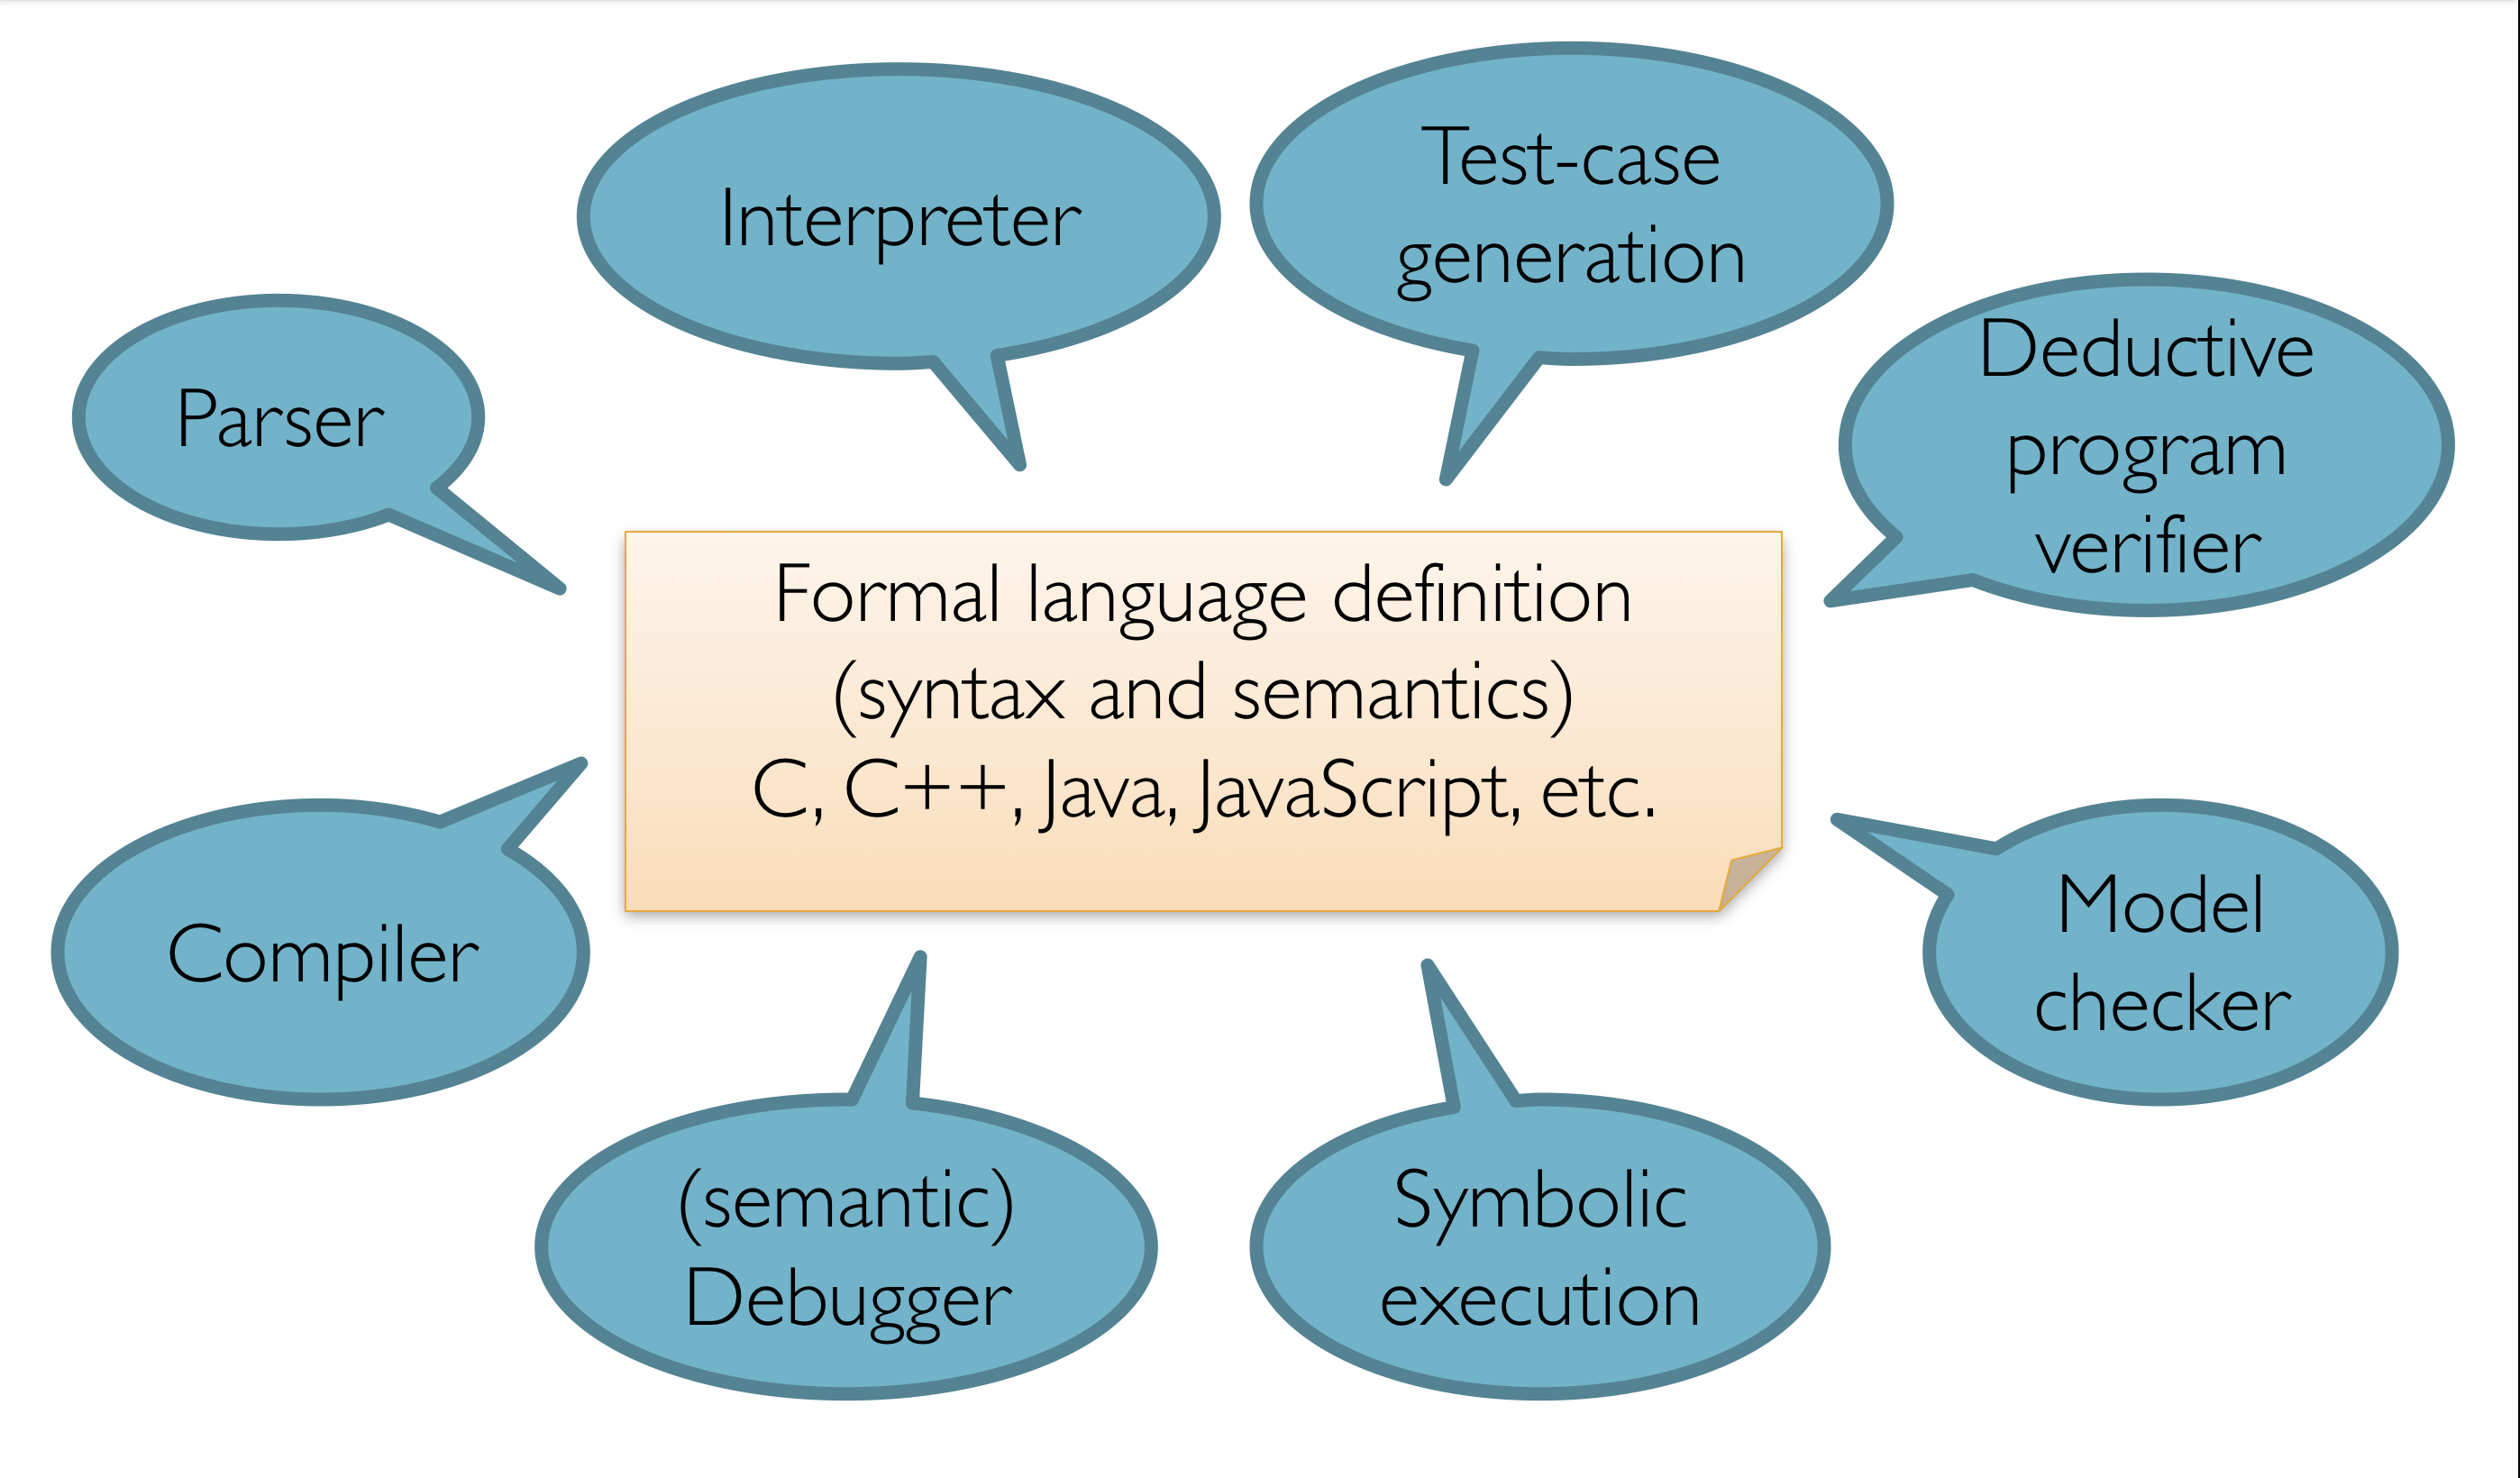
\includegraphics{k-overview.png}
\caption{K Tooling Overview}
\end{figure}

\end{block}

\end{frame}

\begin{frame}{K Backend}

\pause

\begin{block}{Matching Logic}

\begin{itemize}
\tightlist
\item
  Static logic for specifying program configurations.
\item
  Separation Logic and Polyadic Modal Logic are both expressible as ML
  theories.
\end{itemize}

\pause

\end{block}

\begin{block}{Reachability Logic}

\begin{itemize}
\tightlist
\item
  Language independent dynamic logic for reasoning about transition
  systems.
\item
  Sound and relatively complete inference system.
\item
  Generalizes Hoare Logic.
\end{itemize}

\pause

Ask me (or the other team members here) afterwards for more information.

\end{block}

\end{frame}

\begin{frame}[fragile]{K by Example}

\pause

\begin{block}{Github Repositories}

\begin{itemize}
\tightlist
\item
  Organization: \url{https://github.com/kframework}
\item
  KEVM Repository: \url{https://github.com/kframework/evm-semantics}
\item
  All the languages we maintain are developed there.
\item
  In repository \url{https://github.com/kframework/k}, directory
  \texttt{k-distribution/tutorial} has some example toy languages.
\end{itemize}

\pause

In this talk, we'll focus on the KEVM (K semantics of EVM).

\end{block}

\end{frame}

\section{EVM Words}\label{evm-words}

\begin{frame}[fragile]{Utilities}

\pause

\begin{block}{Modulo Arithmetic}

\begin{verbatim}
    syntax Int ::= chop ( Int ) [function]
 // --------------------------------------
    rule chop ( I:Int ) => I %Int pow256
      requires I <Int 0  orBool I >=Int pow256

    rule chop ( I:Int ) => I
      requires I >=Int 0 andBool I <Int pow256
\end{verbatim}

\pause

\end{block}

\begin{block}{Word Arithmetic}

\texttt{\textless{}op\textgreater{}Word} operations incorporate the
behavior for EVM arithmetic:

\begin{verbatim}
    syntax Int ::= Int "+Word" Int [function]
                 | Int "/Word" Int [function]
 // -----------------------------------------
    rule W0 +Word W1 => chop( W0 +Int W1 )
    rule W0 /Word 0  => 0
    rule W0 /Word W1 => chop( W0 /Int W1 ) requires W1 =/=K 0
\end{verbatim}

\end{block}

\end{frame}

\section{\texorpdfstring{Data-Structures over
\texttt{Word}}{Data-Structures over Word}}\label{data-structures-over-word}

\begin{frame}[fragile]{A WordStack for EVM}

\pause

\begin{block}{As a cons-list}

A cons-list is used for the EVM wordstack.

\begin{itemize}
\tightlist
\item
  \texttt{.WordStack} serves as the empty worstack, and
\item
  \texttt{\_:\_} serves as the ``cons'' operator.
\end{itemize}

\begin{verbatim}
    syntax WordStack [flatPredicate]
    syntax WordStack ::= ".WordStack" | Int ":" WordStack
 // -----------------------------------------------------
\end{verbatim}

This can be thought of as a singly linked-list.

\pause

\end{block}

\begin{block}{WordStack Append}

\begin{verbatim}
    syntax WordStack ::= WordStack "++" WordStack [function]
 // --------------------------------------------------------
    rule .WordStack ++ WS' => WS'
    rule (W : WS)   ++ WS' => W : (WS ++ WS')
\end{verbatim}

\end{block}

\end{frame}

\section{EVM Configuration}\label{evm-configuration}

\begin{frame}[fragile]{Keeping Track of World and VM state}

The actual configuration contains \(60+\) cells.

\begin{block}{VM Execution State}

Subconfiguration \texttt{\textless{}evm\textgreater{}} contains the
execution state of a single VM.

\begin{verbatim}
configuration
  <k> $PGM:EthereumSimulation </k>
  <evm>
    <program>   .Map       </program>   // I_b
    <wordStack> .WordStack </wordStack> // \mu_s
    <localMem>  .Map       </localMem>  // \mu_m
    <gas>       0          </gas>       // \mu_g
    ...
  </evm>
  ...
\end{verbatim}

\end{block}

\end{frame}

\begin{frame}[fragile]{Keeping Track of World and VM state}

\begin{block}{Network/World State}

Subconfiguration \texttt{\textless{}network\textgreater{}} contains the
network/world state.

\begin{itemize}
\tightlist
\item
  \texttt{multiplicity="*"} allows for multiple co-existing
  \texttt{\textless{}account\textgreater{}} cells.
\end{itemize}

\begin{verbatim}
configuration
  ...
  <network>
    <activeAccounts> .Map </activeAccounts>
    <accounts>
      <account multiplicity="*" type="Bag">
        <acctID>  0          </acctID>
        <balance> 0          </balance>
        <code>    .WordStack </code>
        <storage> .Map       </storage>
        <nonce>   0          </nonce>
      </account>
    </accounts>
    ...
  </network>
\end{verbatim}

\end{block}

\end{frame}

\section{EVM Execution}\label{evm-execution}

\begin{frame}[fragile]{OpCode Execution}

\pause

\begin{block}{Single Step}

The \texttt{\#next} operator executes a single step by:

\begin{enumerate}
\def\labelenumi{\arabic{enumi}.}
\tightlist
\item
  performing some quick checks for exceptional opcodes,
\item
  executes the opcode if it is not immediately exceptional,
\item
  increments the program counter, and finally
\item
  reverts state if any of the above steps threw an exception.
\end{enumerate}

\pause

\begin{verbatim}
    rule <mode> EXECMODE </mode>
         <k> #next
          => #pushCallStack ~> #exceptional? [ OP ]
                            ~> #exec         [ OP ]
                            ~> #pc           [ OP ]
          ~> #? #dropCallStack : #popCallStack ~> #exception ?#
         ...
         </k>
         <pc> PCOUNT </pc>
         <program> ... PCOUNT |-> OP ... </program>
      requires EXECMODE in (SetItem(NORMAL) SetItem(VMTESTS))
\end{verbatim}

\end{block}

\end{frame}

\section{EVM Programs}\label{evm-programs}

\begin{frame}[fragile]{EVM OpCodes}

\pause

\begin{block}{Expressions}

Expression opcodes call the corresponding
\texttt{\textless{}op\textgreater{}Word} operators, then \texttt{\#push}
the result:

\begin{verbatim}
    syntax BinStackOp ::= "SUB" | "DIV"
 // -----------------------------------
    rule <k> SUB W0 W1 => W0 -Word W1 ~> #push ... </k>
    rule <k> DIV W0 W1 => W0 /Word W1 ~> #push ... </k>
\end{verbatim}

\pause

\end{block}

\begin{block}{Local Memory}

\begin{verbatim}
    syntax UnStackOp ::= "MLOAD"
 // ----------------------------
    rule <k> MLOAD INDEX => #asWord(#range(LM, INDEX, 32)) ~> #push ... </k>
         <localMem> LM </localMem>

    syntax BinStackOp ::= "MSTORE"
 // ------------------------------
    rule <k> MSTORE I V => . ... </k>
         <localMem> LM => LM [ I := #padToWidth(32, #asByteStack(V)) ]
         </localMem>
\end{verbatim}

\end{block}

\end{frame}

\begin{frame}[fragile]{Ethereum Network OpCodes}

\pause

\begin{block}{Account Storage Operations}

These rules reach into the network state and load/store from account
storage:

\begin{verbatim}
    syntax UnStackOp ::= "SLOAD"
 // ----------------------------
    rule <k> SLOAD INDEX => VALUE ~> #push ... </k> <id> ACCT </id>
         <account>
           <acctID> ACCT </acctID>
           <storage> ... INDEX |-> VALUE ... </storage>
           ...
         </account>
\end{verbatim}

\pause

\begin{verbatim}
    syntax BinStackOp ::= "SSTORE"
 // ------------------------------
    rule <k> SSTORE INDEX VALUE => . ... </k> <id> ACCT </id>
         <account>
           <acctID> ACCT </acctID>
           <storage> STORAGE => STORAGE [ INDEX <- VALUE ] </storage>
           ...
         </account>
      requires notBool (INDEX in_keys(STORAGE))
\end{verbatim}

\end{block}

\end{frame}

\begin{frame}[fragile]{Ethereum Network OpCodes}

\pause

\begin{block}{Call Operations}

For each \texttt{CALL*} operation, we make a corresponding call to
\texttt{\#call} and a state-change to setup the custom parts of the
calling environment.

\begin{verbatim}
    syntax CallOp ::= "CALL"
 // ------------------------
    rule <k> CALL GCAP ACCTTO VALUE ARGSTART ARGWIDTH RETSTART RETWIDTH
          => #checkCall ACCTFROM VALUE
          ~> #call ACCTFROM ACCTTO ACCTTO Ccallgas(SCHED, ACCTTO, ACCTS, GCAP, GAVAIL, VALUE) VALUE VALUE #range(LM, ARGSTART, ARGWIDTH)
          ~> #return RETSTART RETWIDTH
         ...
         </k>
         <schedule> SCHED </schedule>
         <id> ACCTFROM </id>
         <localMem> LM </localMem>
         <activeAccounts> ACCTS </activeAccounts>
         <previousGas> GAVAIL </previousGas>
\end{verbatim}

\end{block}

\end{frame}

\section{Ethereum Gas Calculation}\label{ethereum-gas-calculation}

\begin{frame}[fragile]{Execution Gas}

The intrinsic gas calculation mirrors the style of the YellowPaper
(appendix H).

\pause

\begin{block}{SSTORE Gas}

\begin{verbatim}
    syntax InternalOp ::= #gasExec ( Schedule , OpCode )
 // ----------------------------------------------------
    rule <k> #gasExec(SCHED, SSTORE INDEX VALUE)
          => Csstore(SCHED, VALUE, #lookup(STORAGE, INDEX))
         ...
         </k>
         <id> ACCT </id>
         <account>
           <acctID> ACCT </acctID>
           <storage> STORAGE </storage>
           ...
         </account>
\end{verbatim}

\end{block}

\end{frame}

\begin{frame}[fragile]{Gas Calculation Functions}

The following functions are defined in the YellowPaper.

\begin{block}{Csstore}

\begin{verbatim}
    syntax Int ::= Csstore ( Schedule , Int , Int ) [function]
 // ----------------------------------------------------------
    rule Csstore(SCHED, VALUE, OLD)
      => #ifInt VALUE =/=Int 0 andBool OLD ==Int 0
            #then Gsstoreset   < SCHED >
            #else Gsstorereset < SCHED >
         #fi
\end{verbatim}

\pause

\end{block}

\begin{block}{Others}

\begin{verbatim}
    syntax Int ::= Ccall    (Schedule, Int, Map, Int, Int, Int) [function]
                 | Ccallgas (Schedule, Int, Map, Int, Int, Int) [function]
                 | Cgascap  (Schedule, Int, Int, Int)           [function]
                 | Cextra   (Schedule, Int, Map, Int)           [function]
                 | Cxfer    (Schedule, Int)                     [function]
                 | Cnew     (Schedule, Int, Map, Int)           [function]
 // ----------------------------------------------------------------------
\end{verbatim}

\end{block}

\end{frame}

\begin{frame}[fragile]{Fee Schedule from C++ Implementation}

\pause

\begin{block}{Schedule Constants}

A \texttt{ScheduleConst} is a constant determined by the fee schedule.

\begin{verbatim}
    syntax Int ::= ScheduleConst "<" Schedule ">" [function]

    syntax ScheduleConst ::= "Gzero" | "Gbase" | "Gverylow"
 // -------------------------------------------------------
\end{verbatim}

\pause

\end{block}

\begin{block}{Default Schedule}

\begin{verbatim}
    syntax Schedule ::= "DEFAULT"
 // -----------------------------
    rule Gzero < DEFAULT > => 0
    rule Gbase < DEFAULT > => 2
\end{verbatim}

\pause

\end{block}

\begin{block}{EIP150 Schedule}

\begin{verbatim}
    syntax Schedule ::= "EIP150"
 // ----------------------------
    rule Gbalance < EIP150 > => 400
    rule Gsload   < EIP150 > => 200
\end{verbatim}

\end{block}

\end{frame}

\section{The Sum To N Specification}\label{the-sum-to-n-specification}

\begin{frame}[fragile]{Sum To N Program and Claim}

\pause

\begin{block}{High Level}

Canonical ``hello world'' verification example, in no particular
language:

\begin{verbatim}
s = 0;
n = N;
while (n > 0) {
    s = s + n;
    n = n - 1;
}
return s;
\end{verbatim}

\pause

\end{block}

\begin{block}{Claim}

\[s = \sum_{i = 1}^N i = \frac{N * (N + 1)}{2}\]

\end{block}

\end{frame}

\begin{frame}[fragile]{Proof Claims}

\pause

\begin{block}{Main Claim}

\begin{itemize}
\tightlist
\item
  We start at program counter 0 and end at 53.
\item
  The \texttt{\textless{}wordStack\textgreater{}} starts small enough
  and ends with the correct sum.
\item
  The gas consumed is no more than \texttt{(52\ *\ N)\ +\ 27}.
\item
  \texttt{N} is sufficiently low that overflow will not occur in
  execution.
\end{itemize}

\pause

\begin{verbatim}
     <pc>        0  => 53                                </pc>
     <wordStack> WS => 0 : N *Int (N +Int 1) /Int 2 : WS </wordStack>
     <gas>       G  => G -Int (52 *Int N +Int 27)        </gas>

  requires N >=Int 0
   andBool N <=Int 340282366920938463463374607431768211455
   andBool #sizeWordStack(WS) <Int 1021
   andBool G >=Int 52 *Int N +Int 27
\end{verbatim}

\end{block}

\end{frame}

\begin{frame}[fragile]{Proof Claims}

\pause

\begin{block}{Circularity (Loop Invariant)}

We specify the behaviour of the rest of the program any time it reaches
the loop head:

\begin{itemize}
\tightlist
\item
  We start at program counter 35 (beginning of loop) and end at 53.
\item
  \texttt{\textless{}wordStack\textgreater{}} starts with the counter
  \texttt{I} and the partial sum \texttt{S}, and
\item
  \texttt{\textless{}wordStack\textgreater{}} ends with the correct sum.
\item
  The gas consumed for this fragment is no more than
  \texttt{(52\ *\ I)\ +\ 21}.
\item
  \texttt{S} and \texttt{I} are sufficiently low that overflow will not
  occur during execution.
\end{itemize}

\pause

\begin{verbatim}
     <pc> 35 => 53                         </pc>
     <gas> G => G -Int (52 *Int I +Int 21) </gas>

     <wordStack> I : S                               : WS
              => 0 : S +Int I *Int (I +Int 1) /Int 2 : WS </wordStack>

  requires I >=Int 0
   andBool S >=Int 0
   andBool S +Int I *Int (I +Int 1) /Int 2 <Int pow256
   andBool #sizeWordStack(WS) <Int 1021
   andBool G >=Int 52 *Int I +Int 21
\end{verbatim}

\end{block}

\end{frame}

\begin{frame}[fragile]{Verifing ABI compliant contracts}

\pause

\texttt{\#abiCallData} generates ABI compliant \texttt{callData}:

\begin{verbatim}
    syntax WordStack ::= #abiCallData ( String , TypedArgs ) [function]
 // -------------------------------------------------------------------
    rule #abiCallData( FNAME , ARGS ) =>
        #parseByteStack(substrString(
            Keccak256(#generateSignature(FNAME +String "(", ARGS)), 0, 8))
            ++ #encodeArgs(.WordStack | ARGS)
\end{verbatim}

\pause

Here, we generate \texttt{callData} for call the \texttt{transfer}
function:

\begin{verbatim}
<callData>
    #abiCallData("transfer",#address(%ACCOUNT_TO),#uint256(TRANSFER))
</callData>
\end{verbatim}

Note that \texttt{TRANSFER} is a symbolic word,

\end{frame}

\begin{frame}[fragile]{ERC20: Specifying \texttt{transfer}}

\pause

\begin{itemize}
\tightlist
\item
  Execution reaches a \texttt{RETURN} op code
\item
  Account balances are updated correctly if balances are sufficient.
\end{itemize}

\begin{verbatim}
   <k> #execute => (RETURN _ _ ~> _) </k>
   <callData>  #abiCallData("transfer", ...) </callData>
   <accounts>
     <account>
       <storage> (%ACCT_1_BALANCE |-> (B1 => B1 -Int TRANSFER))
                 (%ACCT_2_BALANCE |-> (B2 => B2 +Int TRANSFER))
       </storage>
       ...
     </account>
   </accounts>

  requires TRANSFER >Int 0 andBool TRANSFER <Int pow256
   andBool B1 >=Int 0      andBool B1 <Int pow256
   andBool B2 >=Int 0      andBool B2 <Int pow256
   andBool B2 +Int TRANSFER <Int pow256
   andBool B1 -Int TRANSFER >=Int 0
   andBool #sizeWordStack(WS) <Int 1017
\end{verbatim}

\end{frame}

\section{Other Work}\label{other-work}

\begin{frame}[fragile]{KEVM}

Too much to present here (ask offline).

\begin{block}{Tests}

\begin{itemize}
\tightlist
\item
  Pass all of VMTests (deprecated) and GeneralStateTests.
\item
  Almost passing BlockchainTests.
\item
  Within an order of magnitude the performance of cpp-ethereum.
\end{itemize}

\end{block}

\begin{block}{Verification}

\begin{itemize}
\tightlist
\item
  Verified ERC20 specification over (fixed) HKG Token (see Github
  repository).
\item
  Added ABI-level abstractions for easier specification of proofs (in
  progress).
\end{itemize}

\end{block}

\begin{block}{High Level Languages (not discussed here)}

\begin{itemize}
\tightlist
\item
  \texttt{EVM-PRIME} from IC3 Bootcamp.
\item
  Extending with more primitives to give semantics to Viper.
\end{itemize}

\end{block}

\end{frame}

\begin{frame}{K Framework}

\begin{block}{Language Independent PL/FM Toolkit}

\begin{itemize}
\tightlist
\item
  Parser/interpreter/debugger/model-checker/verification tools all
  exist.
\item
  Work towards semantics-based compiler (for even better performance).
\end{itemize}

\end{block}

\begin{block}{Future Directions}

\begin{itemize}
\tightlist
\item
  More analysis tools built on KEVM.
\item
  Other blockchain language semantics in progress.
\item
  Other (non-blockchain) language/systems/network semantics in progress.
\end{itemize}

\end{block}

\end{frame}

\section{The End}\label{the-end}

\begin{frame}{Acknowledgments}

\begin{itemize}
\tightlist
\item
  Formal Systems Lab (FSL) at UIUC for K support:
  \url{http://fsl.cs.illinois.edu}
\item
  Runtime Verification, Inc. for K support:
  \url{http://runtimeverification.com}
\item
  IOHK for funding and ideas: \url{http://iohk.io}
\item
  Ethereum Foundation/Devcon3 Teams for hosting:
  \url{https://ethereum.org}
\end{itemize}

\end{frame}

\end{document}
